\documentclass[a4paper,12pt]{article} 

%%%%%%%%%%%%%%%%%%%%%%%%%%%%%%%% CONSTANTES %%%%%%%%%%%%%%%%%%%%%%%%%%%%%%%%%%%
\newcommand{\numero}{7}                                    %Numéro de la série -1

\usepackage[french]{babel}
\usepackage[utf8]{inputenc}
\usepackage{answers}

\usepackage{hyperref}
\usepackage{multicol}

\usepackage[table,xcdraw]{xcolor}
\usepackage{listings}
\definecolor{ForestGreen}{RGB}{34,139,34}


\usepackage{enumitem}

\AtBeginDocument{\def\labelitemi{$\bullet$}}


\newcommand{\py}{\lstinline{Python} }


\definecolor{backcolour}{rgb}{0.95,0.95,0.92}

\lstset{%
	language         = Python,
	backgroundcolor  = \color{backcolour},
	basicstyle       = \ttfamily, % \upshape\ttfamily,
	keywordstyle     = \bfseries\color{blue}, %\bfseries,
	stringstyle      = \color{magenta},
	commentstyle     = \color{ForestGreen},
	alsoletter = > ,
	morekeywords = {>>>,as,assert,False,None, nonlocal,True, with,yield , <<, >>, :},
	showstringspaces = false,
	numbers=left,
	stepnumber=1,
	literate={à}{{\`{a}}}1 {é}{{\'e}}1 {è}{{\`{e}}}1 {ê}{{\^{e}}}1 {Ê}{{\^{E}}}1 {î}{{\^i}}1 {ô}{{\^{o}}}1 {ç}{{\c{c}}}1 {Ç}{{\c{C}}}1
}

\newcommand{\itemb}[1]{\item \textbf{#1}}

\usepackage{fancyhdr}  %package pour en-tetes et pied de pages
\usepackage{sectsty} % Permet de faire des modifications de police dans diverses sections des "headings" (cf. modif presentation de la page)
\pagestyle{fancy}       %Style pour en-tetes et pieds de pages
\fancyhead[CO,CE]{\sc Série 1\hspace{0.5mm}}
\fancyhead[RO,LE]{Collège Sismondi}  % LaTeX/TEX define \strut to be an invisible box of width zero that extends just enough above and below the baseline. Cela permet d'augementer légèrement la taille en bas de la box de manière à ce qu'elle soit collée à la ligne.
\fancyhead[LO,RE]{\small\ \textsl{1\textsuperscript{ère} année - DO Informatique}}
\fancyfoot[RO,LE]{2021 - 2022}
\fancyfoot[LO,RE]{\small }
\fancyfoot[CO,CE]{\thepage}

\fancyhfoffset[l]{1.2cm} % le "l" en paramètre permet d'indiquer qu'on ne veut modifier que la marge à gauche.
\renewcommand{\headrule}{{%
		\hrule \headwidth \headrulewidth \vskip-\headrulewidth}}
\renewcommand\footrulewidth{\headrulewidth}
\renewcommand{\footrule}{{%
		\vskip-\footruleskip\vskip-\footrulewidth
		\hrule \headwidth \footrulewidth\vskip\footruleskip}}

\usepackage{tikz}
%-------------------------------------------------------------------------------
%---- Eclairage : en encadré sur fond jaune avec symbôle "ampoule" à gauche ----
%-------------------------------------------------------------------------------
\definecolor{coleclairage}{RGB}{255 , 221 , 156}
\definecolor{contoureclairage}{RGB}{255 , 192 , 0}
\newenvironment{eclairage}
{
	\begin{center}%
		\begin{tikzpicture}%
			\node[rectangle, draw=contoureclairage, top color=coleclairage!50, bottom color=coleclairage!140, rounded corners=5pt, inner xsep=5pt, inner ysep=6pt, outer ysep=10pt]\bgroup                     
			\begin{minipage}{0.98\linewidth}
				\begin{minipage}{0.08\linewidth}\centerline{
\includegraphics[scale=1]{Symbole_eclairage.png}}\end{minipage}
				\begin{minipage}{0.89\linewidth}\itshape\footnotesize
				}
				{                		
				\end{minipage}
			\end{minipage}\egroup;%
		\end{tikzpicture}%
	\end{center}%
}

%-------------------------------------------------------------------------------
%---- apprendre : en encadré sur fond jaune avec symbôle "ampoule" à gauche ----
%-------------------------------------------------------------------------------
\definecolor{colapprendre}{RGB}{50,205,50}
\definecolor{contourapprendre}{RGB}{34,139,34}
\newenvironment{apprendre}
{
	\begin{center}%
		\begin{tikzpicture}%
			\node[rectangle, draw=contourapprendre, top color=colapprendre!10, bottom color=colapprendre!50, rounded corners=5pt, inner xsep=5pt, inner ysep=6pt, outer ysep=10pt]\bgroup                     
			\begin{minipage}{0.98\linewidth}
				\begin{minipage}{0.08\linewidth}\centerline{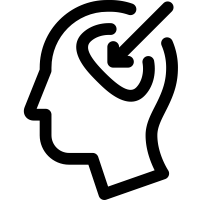
\includegraphics[width=30px]{Symbole_learn.png}}\end{minipage}
				\begin{minipage}{0.89\linewidth}\itshape\footnotesize
				}
				{                		
				\end{minipage}
			\end{minipage}\egroup;%
		\end{tikzpicture}%
	\end{center}%
}

\definecolor{colimportant}{RGB}{247 , 189 , 164}
\definecolor{contourimportant}{RGB}{237 , 125 , 49}
\newenvironment{important}
{
	\begin{center}%
		\begin{tikzpicture}%
			\node[rectangle, draw=contourimportant, top color=colimportant!50, bottom color=colimportant!140, rounded corners=5pt, inner xsep=5pt, inner ysep=6pt, outer ysep=10pt]\bgroup                     
			\begin{minipage}{0.08\linewidth}\centerline{
\includegraphics[scale=0.8]{Symbole_attention.png}}\end{minipage}
			\begin{minipage}{0.89\linewidth}
			}
			{                		
			\end{minipage}\egroup;
		\end{tikzpicture}%
	\end{center}%
}

%-----------------------------------------------------------------
%---- Modification présentation de la page: marges de la page ----
%-----------------------------------------------------------------
%\addtolength{\hoffset}{-1in}              % 1
%\addtolength{\voffset}{-1in}              % 2
\addtolength{\oddsidemargin}{-0.1 in} % 3
\addtolength{\evensidemargin}{-1in} % 3
\addtolength{\topmargin}{-1in}       % 4
\addtolength{\headheight}{6pt}       % 5
%\addtolength{\headsep}{-0.2cm}           % 6
\setlength{\textheight}{26cm}    % 7
\setlength{\textwidth}{16.5cm}      % 8
\addtolength{\marginparsep}{0pt}      % 9
\setlength{\marginparwidth}{0pt}   % 10
\addtolength{\footskip}{-1mm}           %11

\setlength{\parindent}{0em}% pas d'indentation


% Customiser le nom des sections
\usepackage{titlesec}
\titleformat{\section}[hang]{\Large \bfseries}{Série \thesection:\ }{0pt}{}

\renewcommand{\familydefault}{\sfdefault} % pour avoir des polices san serif

\newtheorem{Exc}{Exercice}
\Newassociation{correction}{Soln}{mycor}
\renewcommand{\Solnlabel}[1]{\bfseries Ex #1 }
\def\exo#1{%
	\futurelet\testchar\MaybeOptArgmyexoo}
\def\MaybeOptArgmyexoo{
	\ifx[\testchar \let\next\OptArgmyexoo
	\else \let\next\NoOptArgmyexoo \fi \next}
\def\OptArgmyexoo[#1]{%
	\begin{Exc}[#1]\normalfont}
	\def\NoOptArgmyexoo{%
		\begin{Exc}\normalfont}
		\newcommand{\finexo}{\end{Exc} \vspace{3mm}}
	\newcommand{\flag}[1]{}
	\newcommand{\entete}[1]

\newcommand{\getexocompteur}{{\the\numexpr \arabic{Exc}  \relax}}	
	
\newcommand{\eexo}{\vspace{5mm}} % espace pour séparer les exercices



\begin{document}
%		\title{\vspace{-3cm}Série 1}
%		\date{\vspace{-2cm}}
%		\maketitle

\fancyhead[CO,CE]{\sc Série \arabic{section} \hspace{0.5mm}}

\setcounter{section}{\numero}
\section{Les variables}				
\Opensolutionfile{mycor}[cor_01]

\exo{}  ~\\ 
 Entourer en rouge les noms de variable entraînant une erreur d’exécution et en bleu les noms de variables n’entraînant pas d’erreurs d’exécution mais mal choisis d'après vous.
\begin{multicols}{7}
	{\small
		valeurs\\
		A'\\
		\_zarbi\\
		int\\
		beau\_pere\\
		nb\\
		beauperes\\
		Temp\_Corps \\
		x7\\
		temp-peau\\
		TC\\
		nb\_belle-meres\\
		belle fille\\
		nb\_beau\_fils\\
		Tableau\\
		False\_True\\
		1MA1\_DF07\\
		var\\
		n1
	}
\end{multicols}		
\finexo

\exo{}  ~\\ 
Proposez un nom de variable permettant de stocker :
\begin{itemize}
	\item le nombre de filles de en première OS Math Physique
	\item  le tarif d’un repas à la cafétéria
	\item l’aire d’un triangle (il n’y a qu’une seule figure)
	\item la note à une évaluation d’informatique
\end{itemize}
	\begin{correction}
		~\\ 
		Par exemple, dans les quatre cas:
		\begin{itemize}
			\item \lstinline{nb_filles_1er}
			\item  \lstinline{menu_prix}
			\item  \lstinline{aire_triangle}
			\item  \lstinline{note_eval_info}
		\end{itemize}
	\end{correction}
\finexo

\exo{}  ~\\ 
 Un prof de français à stocké les notes de deux de ses élèves dans les variable \lstinline{n1} et \lstinline{n2}. Le problème c'est qu'il s'est trompé, il doit maintenant permuter le contenu de ces deux variables.   Pour simplifier, on suppose que la variable  \lstinline{n1} stocke le nombre  \lstinline{3}, tandis que la variable  \lstinline{n2} stocke le nombre  \lstinline{5.5}.
\begin{center}
	\vspace{-5mm}
	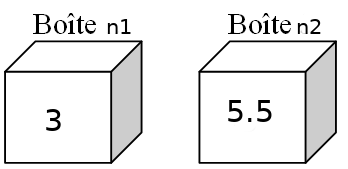
\includegraphics[width=0.3\linewidth]{images/exo_permut.png}
\end{center}
\vspace{-5mm}
\begin{enumerate}
	\item Monsieur Alain Prolo propose l'algorithme suivant :
	\hspace{-8cm}
	\begin{minipage}[t]{0.85\linewidth}
		\begin{lstlisting}
n1 = 3
n2 = 5.5
n1 = n2
n2 = n1
		\end{lstlisting}
	\end{minipage}
	\begin{enumerate}[label=\alph*.]
		\item Compléter sur le tableau d'exécution ci-dessous, en donnant la valeur des variable \lstinline{n1} et \lstinline{n2} après l'exécution de chaque l'instruction numérotée.
		\begin{center}
			\begin{tabular}{|l|p{5cm}|p{5cm}|}
				\hline
				\rowcolor[HTML]{EFEFEF} 
				lignes & Valeur de n1  & Valeur de n2  \\ \hline
				1&         3 &         rien     \\ \hline
				2&          &              \\ \hline
				3&          &              \\ \hline
				4&          &              \\ \hline
				
			\end{tabular}
		\end{center}
		\item Est-ce le programme proposé par Monsieur Alain Prolot permet d'échanger les valeurs stockées dans les variables \lstinline{n1} et de \lstinline{n2} ?
	\end{enumerate}
	\newpage
	
	\item Madame Céline Rasteau propose l'algorithme suivant :
	\hspace{-8.8cm}
	\begin{minipage}[t]{0.85\linewidth}
		\begin{lstlisting}
n1 = 3
n2 = 5.5
n2 = n1
n1 = n2
		\end{lstlisting}
	\end{minipage}
	\begin{enumerate}[label=\alph*.]
		\item Compléter sur le tableau d'exécution ci-dessous, en donnant la valeur des variable \lstinline{n1} et \lstinline{n2} après l'exécution de chaque l'instruction numérotée.
		\begin{center}
			\begin{tabular}{|l|p{5cm}|p{5cm}|}
				\hline
				\rowcolor[HTML]{EFEFEF} 
				lignes & Valeur de n1  & Valeur de n2  \\ \hline
				1&          &              \\ \hline
				2&          &              \\ \hline
				3&          &              \\ \hline
				4&          &              \\ \hline
				
			\end{tabular}
		\end{center}
		\item Est-ce le programme proposé par madame Céline Rasteau permet d'échanger les valeurs stockées dans les variables \lstinline{n1} et de \lstinline{n2} ?		
	\end{enumerate}
	\item  Proposer un programme qui permet d'échanger les valeurs stockées dans les variables \textbf{sans utiliser l'affectation parallèle.}
\end{enumerate}

\begin{correction}
	~\\ 
	\begin{enumerate}
		\item 
		\begin{enumerate}[label=\alph*.]
			\item 
			\begin{center}
				\begin{tabular}{|l|p{5cm}|p{5cm}|}
					\hline
					\rowcolor[HTML]{EFEFEF} 
					lignes & Valeur de n1  & Valeur de n2  \\ \hline
					1&         3 &         rien     \\ \hline
					2&         3  &        5.5      \\ \hline
					3&        5.5  &       5.5       \\ \hline
					4&        5.5  &       5.5       \\ \hline
					
				\end{tabular}
			\end{center}
			\item Non
		\end{enumerate}
		
		\item 
		\begin{enumerate}[label=\alph*.]
			\item Compléter sur le tableau d'exécution ci-dessous, en donnant la valeur des variable \lstinline{n1} et \lstinline{n2} après l'exécution de chaque l'instruction numérotée.
			\begin{center}
				\begin{tabular}{|l|p{5cm}|p{5cm}|}
					\hline
					\rowcolor[HTML]{EFEFEF} 
					lignes & Valeur de n1  & Valeur de n2  \\ \hline
					1&    3      &      Rien        \\ \hline
					2&    3      &     5.5         \\ \hline
					3&    3      &     3         \\ \hline
					4&    3      &      3        \\ \hline
					
				\end{tabular}
			\end{center}
			\item Non	
		\end{enumerate}
		\item  On utilise un variable temporaire:
			\begin{lstlisting}[numbers=none]
n1 = 3
n2 = 5.5
tmp = n1
n1 = n2
n2 = tmp
			\end{lstlisting}
			ou l'affectation multiple
			\begin{lstlisting}[numbers=none]
n1, n2 = n2, n1
			\end{lstlisting}
	\end{enumerate}

\end{correction}
\finexo



\exo{}  ~\\ 
{}  ~\\ 
 On considère le programme dans la colonne Code ci-dessous.
\begin{center}
	\begin{tabular}{|l|l|p{5cm}|}
		\hline
		\rowcolor[HTML]{EFEFEF} 
		lignes & code & Valeur de x  \\ \hline
		1&          x =  0&              \\ \hline
		2&          a = 1&              \\ \hline
		3&          b = 9&              \\ \hline
		4&          c = 4&              \\ \hline
		5&          d = 8&              \\ \hline
		6&          x = a&              \\ \hline
		7&          x = x * 10 + b&              \\ \hline
		8&          x = x * 10 + c&              \\ \hline
		9&          x = x * 10 + d&              \\ \hline
	\end{tabular}
\end{center}

\begin{enumerate}[label=\alph*)]
	\item Compléter la colonne de droite en donnant la valeur courante de la variable x après que la k-ième  ligne ait été exécutée.
	\item Pour vous aider à comprendre le programme, essayer de l'exécuter dans Thonny instruction après instruction en mode débogueur (voir le tutoriel) en regardant l'évolution de la variable x dans la fenêtre \textit{variables}.
\end{enumerate}

\finexo

\newpage

\exo{}  ~\\ 
\begin{enumerate}[label=\alph*)]
	\item  	Indiquez la valeur des variables à l’issue de chaque ligne du programme suivant.
	\begin{lstlisting}[numbers=none]
		a = 4.5
		b = 5
		c = a + b
		d = c / 2
	\end{lstlisting}
	\item 	Quel est le type de chaque variable ?
	\item On considère maintenant que \lstinline{a} et \lstinline{b} correspondent à des notes. Réécrivez le programme en utilisant des noms de variables plus représentatifs (pour les 4 variables).
\end{enumerate}
\begin{correction}
	~\\ 
	
\end{correction}
\finexo


\exo{}  ~\\ 
 On considère le programme \py suivant.
\begin{lstlisting}[numbers=none]
a = 8
b = 3
a = a - 4
b = 2 * b
a = a + b
print(a)
\end{lstlisting}
\begin{enumerate}[label=\alph*)]
	\item  	Combien de variables sont utilisées ?
	\item Quelle est la valeur finale de la variable \lstinline{a} ?
	\item Vérifiez votre réponse à la question précédente en exécutant le code sur Thonny.
	\item Il est possible d’afficher plusieurs valeurs avec la fonction \lstinline{print}. Par exemple, si on veut afficher les valeurs des variables \lstinline{a} et \lstinline{b} on écrit simplement \lstinline{print(a, b)}. Modifiez la dernière ligne du programme et exécutez-le.
\end{enumerate}
\finexo

\exo{}  ~\\ 
 On considère le programme \py suivant.
\begin{lstlisting}[numbers=none]
a = 5
b = a + 1
b = b + 2
c = b - a
print(c)
\end{lstlisting}
\begin{enumerate}[label=\alph*)]
	\item  	Qu’affiche ce programme ?
	\item Vérifiez votre réponse à la question précédente en exécutant le code sur Thonny.
\end{enumerate}
\begin{correction}
	~\\ 
	\lstinputlisting{codes/ex8.py}
\end{correction}
\finexo

\exo{}  ~\\ 
 Écrire un programme qui initialise une variable appelée \lstinline{a} avec la valeur 6, puis affiche le contenu de \lstinline{a}, la divise par trois et la remet dans \lstinline{a} et finalement affiche la nouvelle valeur de \lstinline{a} à l'écran.

\finexo

\newpage
\exo{}  ~\\ 
 Est-ce que les 4 scripts (petits programmes) sont valides? Si oui que s’affichera-t-il à l’écran? Dans le cas contraire, expliquer ce qui ne va pas.  
\begin{multicols}{2}
	\begin{lstlisting}[numbers=none]
a, b = 'Mahe', 'Moeve'
print('a = ', a, ' et b = ', b)
	\end{lstlisting}
	\begin{lstlisting}[numbers=none]
		
a = b
b = 1
print('a = ', a, ' et b = ', b)
	\end{lstlisting}
	\begin{lstlisting}[numbers=none]
a, b = Mahe, Moeve
print('a = ', a, ' et b = ', b)
	\end{lstlisting}
	\begin{lstlisting}[numbers=none]
a, b = 2, 3
a = b
b = a
print('a = ', a, ' et b = ', b)
	\end{lstlisting}
\end{multicols}
\vspace{-5mm}
Exécuter ces programme avec Thonny afin de vérifier si vos réponses sont correctes.

\begin{important}
	Avant de pouvoir utiliser une variable il faut toujours la déclarer, c'est-à-dire en \py faire une affectation à la variable avec une valeur valide
\end{important}

\finexo

\exo{}  ~\\ 
 On considère le programme de calcul suivant.
\begin{itemize}
	\item \lstinline{a} prend la valeur 5
	\item  Multiplier \lstinline{a}  par 3
	\item Soustraire 4 au résultat
	\item Elever le résultat au carré
	\item Afficher le résultat
\end{itemize}
Ecriver un programme Python permettant de coder ce programme de calcul.
\begin{correction}
	~\\ 
	\lstinputlisting{codes/ex10.py}
\end{correction}
\finexo

\begin{apprendre}
	Pour demander à l’utilisateur de déterminer le contenu d’une variable, on utilise l’instruction \lstinline{input}.
	\begin{lstlisting}[numbers=none]
prenom=input("quel est ton prenom? ")
print(prenom)
	\end{lstlisting}
	Par défault la fonction \lstinline{input} retourne une chaîne de caractère. Si l'on souhaite demander à l'utilisateur un nombre, il faut entourner la fonction \lstinline{input} du type souhaité
	\begin{lstlisting}[numbers=none]
age = int(input("quel est ton age? "))        # age sera de type int
taille = int(input("quel est ta taille? "))   # taille sera de type float
print("j'ai ", age, " et je mesure ", taille)  
	\end{lstlisting}
\end{apprendre}

\exo{}  ~\\ 
 Écrire un script en Python qui demande à l'utilisateur, son prénom, son nom et son âge et qui réalise un affichage du type \lstinline{"Bonjour je m'appelle Rene Descartes, j'ai 425 ans!"}.
 \begin{correction}
 	~\\ 
 	\lstinputlisting{codes/ex11.py}
 \end{correction}
\finexo

\newpage

\exo{}  ~\\ 
  Un boulanger désire un programme qui demande à l'utilisateur le nombre de baguettes qu'il désire, qui calcule le prix total (sachant qu'une baguette coûte 2.50CHF) et qui affiche le prix que l'utilisateur doit payer. 
\begin{enumerate}[label=\alph*)]
	\item  	Testez le script suivant :
	\begin{lstlisting}[numbers=none]
nombre=input("Combien de baguettes désirez-vous ?")
prix = nombre * 1.1
print("Vous avez à payer",prix,"euros.")
	\end{lstlisting}
	\item Quel message d'erreur obtenez-vous ?
	
	\item Modifier le code ci-dessus pour que le programme fonctionne.
\end{enumerate}
\begin{correction}
	~\\ 
	\begin{enumerate}[label=\alph*)]
		\item  	\ 

		\item Un problème de type
		
		\item 
		\begin{lstlisting}[numbers=none]
nombre=float(input("Combien de baguettes désirez-vous ?"))
prix = nombre * 1.1
print("Vous avez à payer",prix,"euros.")
		\end{lstlisting}
	\end{enumerate}
\end{correction}
\finexo

\exo{}  ~\\ 
  L'Indice de Masse Corporelle (IMC) est un indicateur chiffré utilisé en médecine. L'IMC d'une personne est donné par la formule $IMC = \frac{masse}{taille ^2}$  où la masse est en kilos et la taille en mètres. 

Proposer un algorithme qui demande à l'utilisateur sa taille et sa masse puis qui affiche l'IMC de la personne. 
\begin{correction}
	~\\ 
	\lstinputlisting{codes/ex13.py}
\end{correction}
\finexo

\exo{}[Apprendre en  autonomie avec france IOI]  ~\\ 
Allez sur le site de france IOI sur \url{http://www.france-ioi.org/}, puis valider la séquence 3 "\textit{Calculs et découverte des variables}".
\finexo

% Solution		
		\newpage
		\setcounter{page}{1}
		\setcounter{section}{\numero}
		\Closesolutionfile{mycor}
		\titleformat{\section}[hang]{\Large \bfseries}{Corrigé Série \thesection:\ }{0pt}{}
		

		\fancyhead[CO,CE]{\sc Corrigé Série \arabic{section} \hspace{0.5mm}}
		\section{}
		\Readsolutionfile{mycor}
	\end{document}